\section{Operation of the Currency Input Circuit}

\subsection{Initialization}
\begin{enumerate}
\item After powering on the circuit, reset all of the flip flops to ensure that their value is zero. If this is not done, a user can continuously reboot the machine and collect an amount of change equal to the value of the flip flops as they are powered on. Since they are not guaranteed to initialize to a 1 or 0, skipping this step could lead to losing a lot of money. 
\end{enumerate}

\subsection{How to Record an Accepted Bill}
\begin{enumerate}
\item Since we do not have an actual bill reader, we need to set the number of dollars being inserted using switches 1 through 6. These correspond to inputs $B_0$ through $B_5$ to the ALU.
\item While the selector bit is set to addition, generate a single clock pulse by pressing the upper button followed by the lower button.
\item On the falling edge, the flip flops will be set to the sum of the input and the value that is already stored in the flip flops. 
\end{enumerate}

\begin{figure}[H]
\centering
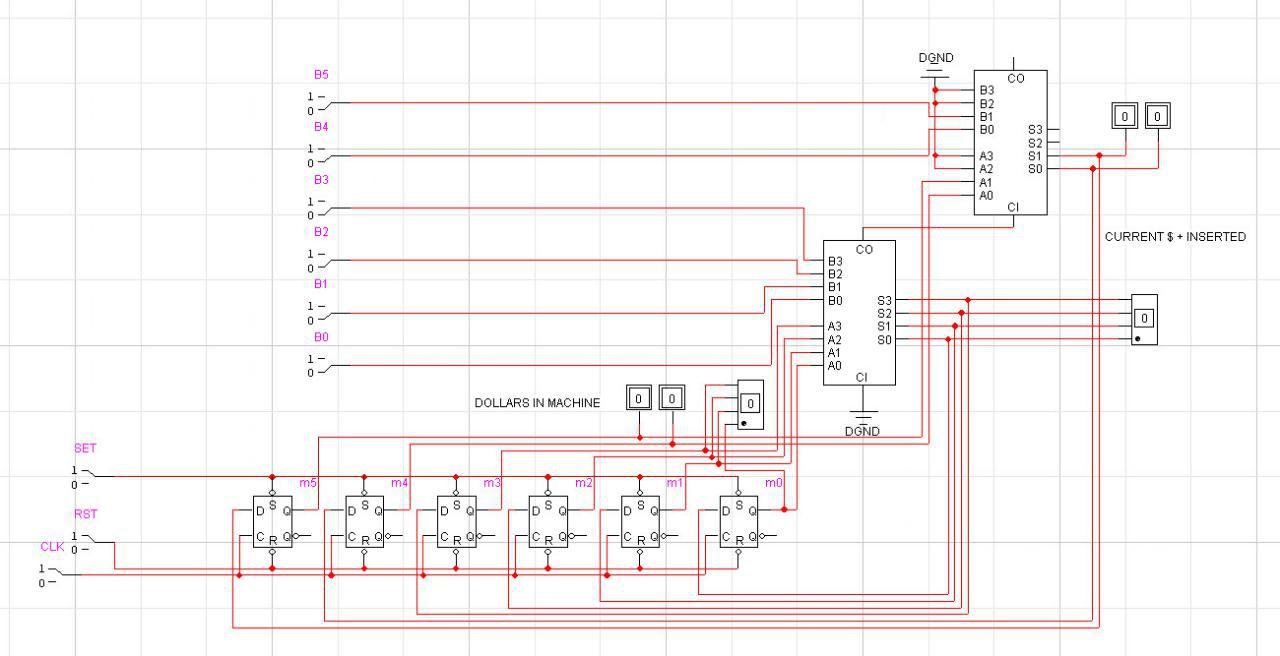
\includegraphics[width=16.5cm]{input} \\
%\vspace{1em} \hspace{1em}
\caption{This is the completed input circuit. 4-bit adders (74LS83) are used in the circuit diagram instead of 4-bit ALUs (74\_181) to simplify the diagram. In the actual implementation, the adders are replaced with ALUs.}
\label{input-circuit}
\end{figure}
